\documentclass{scrartcl}
\usepackage{tikz}
\usetikzlibrary{calc}

\begin{document}

\tikzset{
    every node/.style={
        circle,
        draw,
        solid,
        fill=black,
        inner sep=0pt,
        minimum width=4pt
    }
}

\begin{tikzpicture}
  % \node (A) {A};
  \coordinate (1) at (0,0);
  \coordinate (2) at ($(1)+(30:1)$);
  \draw (1) node {} -- (2) node {};  
  % \draw (2) node {} -- ++(50:1) node {};
  % \draw (1) node {} -- ++(30:2) node {};  
  % \path (A) ++(30:2) node (B) [draw,fill=blue!20] {B};
\end{tikzpicture}

\begin{tikzpicture}
  % \node (A) {A};
  \def\prev{0} % Variable to store the previous element
  \def\numbers{1,2,3,4,5}
  \def\angle{30}
  \coordinate (\prev) at (0,0);
  \foreach \curr in \numbers{
    \coordinate (\curr) at ($(\prev)+(\angle:1)$);
    \draw (\prev) node {} -- (\curr) node {};      
    \xdef\prev{\curr} % Update the previous element to the current element
  }

  \def\prev{0} % Variable to store the previous element  
  \def\numbers{6,7,8}
  \foreach \curr in \numbers{
    \coordinate (\curr) at ($(\prev)+(-30:1)$);
    \draw (\prev) node {} -- (\curr) node {};      
    \xdef\prev{\curr} % Update the previous element to the current element
  }
  
  % \coordinate (2) at ($(1)+(30:1)$);
  % \draw (1) node {} -- (2) node {};  
  % \draw (2) node {} -- ++(50:1) node {};
  % \draw (1) node {} -- ++(30:2) node {};  
  % \path (A) ++(30:2) node (B) [draw,fill=blue!20] {B};
\end{tikzpicture}


  
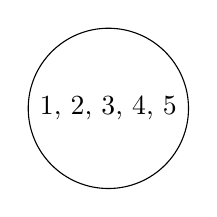
\begin{tikzpicture}
    % Define a list of numbers
    \def\numbers{{1, 2, 3, 4, 5}}
    
    % Loop through the list of numbers
    \foreach \curr in \numbers {
        \node[circle, draw] at (\curr, 0) {\curr}; % Create a node with the current number
    }
  \end{tikzpicture}

  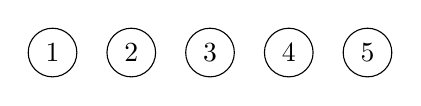
\begin{tikzpicture}
    \def\prev{0} % Variable to store the previous element
    \def\numbers{1,2,3,4,5}
    % \pgfmathparse{\numbers[1-1]}
    % \edef\prev{\pgfmathresult}    
    % Loop through a list of numbers
    \foreach \curr in \numbers{
        \node[circle, draw] (\curr) at (\prev, 0) {\curr}; % Create a node with the current number
        \xdef\prev{\curr} % Update the previous element to the current element
    }
\end{tikzpicture}

\end{document}